% Options for packages loaded elsewhere
\PassOptionsToPackage{unicode}{hyperref}
\PassOptionsToPackage{hyphens}{url}
\documentclass[
  10pt,
  a4paper,
]{article}
\usepackage{xcolor}
\usepackage[margin=22mm]{geometry}
\usepackage{amsmath,amssymb}
\setcounter{secnumdepth}{-\maxdimen} % remove section numbering
\usepackage{iftex}
\ifPDFTeX
  \usepackage[T1]{fontenc}
  \usepackage[utf8]{inputenc}
  \usepackage{textcomp} % provide euro and other symbols
\else % if luatex or xetex
  \usepackage{unicode-math} % this also loads fontspec
  \defaultfontfeatures{Scale=MatchLowercase}
  \defaultfontfeatures[\rmfamily]{Ligatures=TeX,Scale=1}
\fi
\usepackage{lmodern}
\ifPDFTeX\else
  % xetex/luatex font selection
\fi
% Use upquote if available, for straight quotes in verbatim environments
\IfFileExists{upquote.sty}{\usepackage{upquote}}{}
\IfFileExists{microtype.sty}{% use microtype if available
  \usepackage[]{microtype}
  \UseMicrotypeSet[protrusion]{basicmath} % disable protrusion for tt fonts
}{}
\makeatletter
\@ifundefined{KOMAClassName}{% if non-KOMA class
  \IfFileExists{parskip.sty}{%
    \usepackage{parskip}
  }{% else
    \setlength{\parindent}{0pt}
    \setlength{\parskip}{6pt plus 2pt minus 1pt}}
}{% if KOMA class
  \KOMAoptions{parskip=half}}
\makeatother
\usepackage{graphicx}
\makeatletter
\newsavebox\pandoc@box
\newcommand*\pandocbounded[1]{% scales image to fit in text height/width
  \sbox\pandoc@box{#1}%
  \Gscale@div\@tempa{\textheight}{\dimexpr\ht\pandoc@box+\dp\pandoc@box\relax}%
  \Gscale@div\@tempb{\linewidth}{\wd\pandoc@box}%
  \ifdim\@tempb\p@<\@tempa\p@\let\@tempa\@tempb\fi% select the smaller of both
  \ifdim\@tempa\p@<\p@\scalebox{\@tempa}{\usebox\pandoc@box}%
  \else\usebox{\pandoc@box}%
  \fi%
}
% Set default figure placement to htbp
\def\fps@figure{htbp}
\makeatother
\setlength{\emergencystretch}{3em} % prevent overfull lines
\providecommand{\tightlist}{%
  \setlength{\itemsep}{0pt}\setlength{\parskip}{0pt}}
\usepackage{mathrsfs}
\usepackage{mathtools}
\usepackage{xurl}
\emergencystretch=3em
\setcounter{tocdepth}{1}
\newcommand{\Beta}{\mathrm{B}}
\DeclareUnicodeCharacter{00B2}{\ensuremath{^2}}
\DeclareUnicodeCharacter{00B1}{\ensuremath{\pm}}
\DeclareUnicodeCharacter{00D7}{\ensuremath{\times}}
\DeclareUnicodeCharacter{2192}{\ensuremath{\to}}
\DeclareUnicodeCharacter{21A6}{\ensuremath{\mapsto}}
\DeclareUnicodeCharacter{2208}{\ensuremath{\in}}
\DeclareUnicodeCharacter{2209}{\ensuremath{\notin}}
\DeclareUnicodeCharacter{2212}{\ensuremath{-}}
\DeclareUnicodeCharacter{2227}{\ensuremath{\wedge}}
\DeclareUnicodeCharacter{2228}{\ensuremath{\vee}}
\DeclareUnicodeCharacter{2260}{\ensuremath{\ne}}
\DeclareUnicodeCharacter{2264}{\ensuremath{\le}}
\DeclareUnicodeCharacter{2265}{\ensuremath{\ge}}
\DeclareUnicodeCharacter{2297}{\ensuremath{\otimes}}
\usepackage{bookmark}
\IfFileExists{xurl.sty}{\usepackage{xurl}}{} % add URL line breaks if available
\urlstyle{same}
\hypersetup{
  hidelinks,
  pdfcreator={LaTeX via pandoc}}

\author{}
\date{}

\begin{document}

{
\setcounter{tocdepth}{3}
\tableofcontents
}
\section{The ES quarter spectrum, its tetrahedral metric, and the
original heat
trace}\label{the-es-quarter-spectrum-its-tetrahedral-metric-and-the-original-heat-trace}

This note starts with the actual four raw ES cells and their
quarter-inversion operator. It constructs a form-preserving linear
isomorphism with two positive scalar directions and the reflected trace
of the original quadratic heat family. It proves the transported
symmetry actions, the precise multiplication maps, and the surviving
collision algebra. The ES form is not presumed to be the complete Weil
form.

The original source read for this calculation is
\texttt{ES-\allowbreak{}Fable-\allowbreak{}C123/\allowbreak{}es\_\allowbreak{}fable\_\allowbreak{}c123\_\allowbreak{}preprint.\allowbreak{}tex}: the definition
\texttt{eq:\allowbreak{}Hermitian-\allowbreak{}circle-\allowbreak{}coefficients}; Corollaries
\texttt{cor:\allowbreak{}raw-\allowbreak{}blade-\allowbreak{}cells-\allowbreak{}quarter-\allowbreak{}three-\allowbreak{}plus-\allowbreak{}one} and the following
raw-cell projector corollary, including
\texttt{eq:\allowbreak{}four-\allowbreak{}cell-\allowbreak{}explicit-\allowbreak{}quarter-\allowbreak{}images},
\texttt{eq:\allowbreak{}raw-\allowbreak{}negative-\allowbreak{}cell-\allowbreak{}projector},
\texttt{eq:\allowbreak{}raw-\allowbreak{}positive-\allowbreak{}cell-\allowbreak{}projector}; Theorem
\texttt{thm:\allowbreak{}Fable-\allowbreak{}D3-\allowbreak{}raw-\allowbreak{}cell-\allowbreak{}action}; Corollary
\texttt{cor:\allowbreak{}Fable-\allowbreak{}three-\allowbreak{}character-\allowbreak{}tetrahedron}; Theorem
\texttt{thm:\allowbreak{}Fable-\allowbreak{}forced-\allowbreak{}regular-\allowbreak{}four-\allowbreak{}simplex}; and
\texttt{eq:\allowbreak{}quarter-\allowbreak{}inversion-\allowbreak{}matrix} through
\texttt{eq:\allowbreak{}quarter-\allowbreak{}negative-\allowbreak{}eigenline}. These are actual passages of the
source, rather than identifications inferred from a four-element count.
The receiving programme proof read in full is
\href{HEAT_ENDPOINT_SIGN_BRIDGE.md}{the complete heat endpoint sign
bridge proof}, HEB1--HEB32. The original heat equations also have the
public proof
\href{https://github.com/KokunoYumeto/zeta-function-research-reader/blob/ac168d55cbb400a6c8926a00d67909ba65646ac5/satellites/26_incompressible_fibre_heat.tex\#L389}{\emph{The
original heat trajectories}, \texttt{eq:\allowbreak{}ifh-\allowbreak{}target-\allowbreak{}flow} and the ensuing
trajectories}, while
\href{https://github.com/KokunoYumeto/zeta-function-research-reader/blob/173dbc6ed5a03235dbe7654f928f3692107db39b/workbenches/splitzero-tandem/branches/tau-zero-prime-positivity/ESCAPING_FIBRE_INFINITESIMAL_DERIVATION.md\#L89}{EFI7--EFI15}
give their projective graph and collision algebra. All
finite-dimensional claims made below have their proofs here.

\subsection{1. The source operator and its complete
intertwiner}\label{the-source-operator-and-its-complete-intertwiner}

Let \[
V=M_2(\mathbb R),\qquad
x=x_{11}E_{11}+x_{12}E_{12}+x_{21}E_{21}+x_{22}E_{22},
\tag{ESQ1}
\] with the displayed ordering of the four basis vectors. We retain both
the vector space and its original matrix multiplication. The symbol
\(I_2=E_{11}+E_{22}\) denotes the matrix identity, whereas \(I_V\)
denotes the identity linear operator on the four-dimensional vector
space.

The quarter-inversion operator pulled back from the ES source is \[
A_0=\operatorname{diag}(1/4,1/4,-1/4,1/4).
\tag{ESQ2}
\] Its two invariant spaces and its negative projector are \[
U_+=\operatorname{span}_{\mathbb R}\{E_{11},E_{12},E_{22}\},
\quad U_-=\mathbb RE_{21},\qquad
P_-x=x_{21}E_{21}=\left(\frac12I_V-2A_0\right)x.
\tag{ESQ3}
\] These formulas follow by evaluating the diagonal operator on all four
basis vectors. In particular \(P_-^2=P_-\), its kernel is \(U_+\), and
its image is \(U_-\).

Here is the full source intertwiner, including its inverse. In Hermitian
coefficient coordinates write \[
H(\alpha,\beta_0,\beta_1,\gamma)
=\begin{pmatrix}\alpha&\beta_0+i\beta_1\\
\beta_0-i\beta_1&\gamma\end{pmatrix}.
\tag{ESQ4}
\] The coefficient vector of \(\mathcal T_\square x\) is \[
\begin{aligned}
\alpha&=x_{11}+2x_{21}+x_{22},&
\beta_0&=(x_{11}-x_{22})/2,\\
\beta_1&=x_{12},&
\gamma&=(x_{11}+x_{22})/4-x_{21}/2.
\end{aligned}
\tag{ESQ5}
\] This is exactly the linear extension of the four source images. Its
inverse is \[
x_{11}=\alpha/4+\gamma+\beta_0,\quad
x_{22}=\alpha/4+\gamma-\beta_0,\quad
x_{12}=\beta_1,\quad x_{21}=\alpha/4-\gamma.
\tag{ESQ6}
\] Substitution in either direction returns all four starting
coefficients, proving that it is an isomorphism of real vector spaces.
The source coefficient inversion is \[
\mathcal I_-=
\begin{pmatrix}
0&0&0&1\\0&1/4&0&0\\0&0&1/4&0\\1/16&0&0&0
\end{pmatrix}.
\tag{ESQ7}
\] Applying this matrix to the four columns of (ESQ5) multiplies the
\(E_{21}\) column by \(-1/4\) and each other column by \(1/4\). Since
the four columns form a basis, this proves the entire operator identity
\[
\mathcal T_\square A_0=\mathcal I_-\mathcal T_\square.
\tag{ESQ8}
\] The negative line is therefore the specific raw \(E_{21}\) line, not
an unspecified member of a quartet. In the source channel order
\((++),(+-),(-+),(--)\), it is the \((-,+)\) channel. The source
specializations \(\mathcal M(53)=2E_{21}\) and
\(\mathcal M(109)=E_{12}\) retain their different eigenspaces under
(ESQ8).

\subsection{2. The tetrahedral metric and the rank-one heat
motion}\label{the-tetrahedral-metric-and-the-rank-one-heat-motion}

Retain the source's forced metric \[
G=\widehat G_{\mathrm F}=
\begin{pmatrix}
1/16&0&0&-7/144\\
0&2/9&0&0\\
0&0&1&0\\
-7/144&0&0&1/16
\end{pmatrix}.
\tag{ESQ9}
\] On \(U_+\), the sum and difference of \(E_{11},E_{22}\) have
respective eigenvalues \(1/72,1/9\), and \(E_{12}\) has eigenvalue
\(2/9\). The orthogonal fourth direction \(E_{21}\) has eigenvalue 1.
These four positive numbers prove that \(G\) is positive definite. Its
tetrahedral origin is proved again in Section 7.

Use the original forward heat parameter with its original constants, \[
a(h)=-\frac14+2h,\qquad h\in\mathbb R.
\tag{ESQ10}
\] Define the actual deformation of the source operator by \[
A_h=A_0+2hP_-
=\frac14(I_V-P_-)+a(h)P_-.
\tag{ESQ11}
\] It is \(G\)-self-adjoint: the decomposition \(U_+\oplus U_-\) is
\(G\)-orthogonal, and the operator is scalar on each summand.
Equivalently \(A_h^{\mathsf T}G=GA_h\), as is also immediate from the
displayed matrices. Consequently \[
B_h(x,y)=x^{\mathsf T}GA_hy
\tag{ESQ12}
\] is a symmetric bilinear form. Its full matrix and quadratic
expression are \[
GA_h=
\begin{pmatrix}
1/64&0&0&-7/576\\
0&1/18&0&0\\
0&0&a(h)&0\\
-7/576&0&0&1/64
\end{pmatrix},
\tag{ESQ13}
\] \[
B_h(x,x)=\frac{x_{11}^2+x_{22}^2}{64}
-\frac7{288}x_{11}x_{22}
+\frac{x_{12}^2}{18}+a(h)x_{21}^2.
\tag{ESQ14}
\] Matrix multiplication proves every coefficient. The unchanged
positive eigenvalues of this matrix are \(1/288,1/36,1/18\), and its
remaining eigenvalue is \(a(h)\). Thus it has signature \((3,1)\) for
\(h<1/8\), has three positive directions and radical \(\mathbb RE_{21}\)
for \(h=1/8\), and is positive definite for \(h>1/8\). At \(h=1/4\),
\(A_h=I_V/4\) and \(B_h=G/4\). The exact difference formula is \[
B_{h_2}(x,y)-B_{h_1}(x,y)
=2(h_2-h_1)x_{21}y_{21}.
\tag{ESQ15}
\] This follows because \(GP_-=P_-\). It proves that the entire changing
part has rank one and is increasing as a quadratic form when heat time
increases.

For the two marked source specializations this gives the exact values \[
B_h(\mathcal M(53),\mathcal M(53))=4a(h)=-1+8h,
\qquad
B_h(\mathcal M(109),\mathcal M(109))=1/18.
\tag{ESQ15a}
\] They follow from \(\mathcal M(53)=2E_{21}\),
\(\mathcal M(109)=E_{12}\), and (ESQ13), retaining the factor two on the
first source vector.

The original intertwiner also transports the entire heat family, not
only its initial value. Define \[
\mathcal I_h=\mathcal I_-+2h\left(\frac12I-2\mathcal I_-\right)
=hI+(1-4h)\mathcal I_-.
\tag{ESQ16}
\] Substitution of (ESQ3) in (ESQ8) proves
\(\mathcal T_\square A_h=\mathcal I_h\mathcal T_\square\). Transport the
metric by
\(G_T=(\mathcal T_\square^{-1})^{\mathsf T}G\mathcal T_\square^{-1}\).
In the coordinates of (ESQ4) its quadratic expression is \[
G_T(y,y)=\frac{(\alpha+4\gamma)^2}{576}
+\frac29(\beta_0^2+\beta_1^2)+(\alpha/4-\gamma)^2.
\tag{ESQ17}
\] This is obtained by inserting (ESQ6) in (ESQ9). It proves the metric
transport exactly; no identification with the Lorentz form \(-\det H\)
is being substituted for it. Likewise the transported heat form is \[
B_{T,h}(y,y)=\frac{(\alpha+4\gamma)^2}{2304}
+\frac{\beta_0^2+\beta_1^2}{18}
+a(h)(\alpha/4-\gamma)^2.
\tag{ESQ18}
\]

\subsection{3. The exact trace receiver and the form-preserving
isomorphism}\label{the-exact-trace-receiver-and-the-form-preserving-isomorphism}

For real \(a\), let \[
E_a=\mathbb R[r]/(r^2+a).
\tag{ESQ19}
\] Every element has a unique expression \(c+dr\), by division by the
monic quadratic. The real algebra involution is \((c+dr)^\#=c-dr\). It
preserves the relation and squares to the identity. The regular trace is
the trace of multiplication on the basis \((1,r)\). Since \[
L_r=\begin{pmatrix}0&-a\\1&0\end{pmatrix},
\qquad \operatorname{Tr}_{E_a}(c+dr)=2c,
\tag{ESQ20}
\] the full reflected trace pairing is \[
\frac12\operatorname{Tr}_{E_a}((c+dr)^\#(e+fr))=ce+a df.
\tag{ESQ21}
\] Indeed the product has scalar coefficient \(ce+a df\), and (ESQ20)
gives twice it. At complex coefficients the involution also conjugates
\(c,d\), and the same proof gives \(\overline c e+a\overline d f\).

Define the real vector space \[
W_a=\mathbb R^2\oplus E_a
\tag{ESQ22}
\] with symmetric form \[
Q_a((z_1,z_2,p),(t_1,t_2,q))
=z_1t_1+z_2t_2+\frac12\operatorname{Tr}_{E_a}(p^\#q).
\tag{ESQ23}
\] The map proposed for the raw ES cells is exactly \[
\begin{aligned}
\Theta_h:V&\longrightarrow W_{a(h)},\\
z_1&=\frac{x_{11}+x_{22}}{24},\qquad
z_2=\frac{x_{11}-x_{22}}{6\sqrt2},\\
p&=c+dr=\frac{x_{12}}{3\sqrt2}+x_{21}r.
\end{aligned}
\tag{ESQ24}
\] It is a vector-space isomorphism for every \(h\), including the
collision. Its inverse is \[
x_{11}=12z_1+3\sqrt2z_2,\quad
x_{22}=12z_1-3\sqrt2z_2,\quad
x_{12}=3\sqrt2c,\quad x_{21}=d.
\tag{ESQ25}
\] These formulas are mutually inverse by substitution, without dividing
by \(a\). They prove in particular that no vector is dropped when
\(a=0\).

The exact isometry identity is \[
B_h(x,y)=Q_{a(h)}(\Theta_hx,\Theta_hy).
\tag{ESQ26}
\] For the diagonal terms, (ESQ21) gives
\(c^2+a d^2=x_{12}^2/18+a x_{21}^2\). The remaining two squares are \[
\frac{(x_{11}+x_{22})^2}{576}
+\frac{(x_{11}-x_{22})^2}{72}
=\frac{x_{11}^2+x_{22}^2}{64}-\frac7{288}x_{11}x_{22}.
\tag{ESQ27}
\] Expansion proves the equality with (ESQ14). For two arguments the
identical expansion with products proves (ESQ26), or it follows by real
polarization. Complex-linear extension gives the corresponding Hermitian
identity, with all squared terms replaced by absolute squares and first
coefficients conjugated.

The scalar factor one half in (ESQ23) is essential: HEB16 uses the full
regular trace. More precisely, if the whole HEB rank-three form is \[
q_a^{\mathrm{full}}(v,p)=|v|^2+\operatorname{Tr}_{E_a}(p^\#p),
\] then the explicit map \[
(z_1,z_2,p)\longmapsto\bigl(z_1,(z_2,p/\sqrt2)\bigr)
\tag{ESQ28}
\] is an isometry from \(Q_a\) to one additional positive scalar form
plus \(q_a^{\mathrm{full}}\). Its inverse multiplies the last coordinate
by \(\sqrt2\). This gives the exact relation with HEB's whole finite
receiver while retaining the additional positive dimension.

The raw involution \(4A_0=I_V-2P_-\) is also intertwined: \[
\Theta_h(4A_0x)=(z_1,z_2,p^\#)
\quad\text{over real coefficients}.
\tag{ESQ29}
\] Over complex coefficients the matching conjugate-linear raw
involution is \((I_V-2P_-)\overline x\). Each formula follows because
exactly \(x_{21}\) changes sign, with coefficient conjugation added in
the latter case. The heat operator itself becomes the diagonal map \[
(z_1,z_2,c,d)\longmapsto(z_1/4,z_2/4,c/4,a(h)d).
\tag{ESQ30}
\] Under the same coordinates the fixed positive metric is
\(4|z_1|^2+4|z_2|^2+4|c|^2+|d|^2\). This is obtained from \(G\) by
(ESQ25), and together with (ESQ30) reproduces \(Q_a\).

The trace-factor projection and its kernel are completely explicit: \[
0\longrightarrow\operatorname{span}\{E_{11},E_{22}\}
\longrightarrow V\xrightarrow{\ \pi_h\ }E_{a(h)}
\longrightarrow0,
\qquad
\pi_h(x)=x_{12}/(3\sqrt2)+x_{21}r.
\tag{ESQ31}
\] It is onto with linear section \(c+dr\mapsto3\sqrt2cE_{12}+dE_{21}\),
and its kernel follows from the independence of \(1,r\). The kernel is
orthogonal to that section for \(B_h\), and carries the two positive
squares (ESQ27). All assertions hold at the collision as well.

\subsection{4. The endpoint algebra and the changing spectral
pair}\label{the-endpoint-algebra-and-the-changing-spectral-pair}

The exact all-parameter polynomial map to the HEB endpoint family is \[
\mathbb R[s]/(s(s-1)+2h)\xrightarrow{\sim}E_{a(h)},
\qquad s\longmapsto\frac12+r,
\quad\text{inverse: }r\longmapsto s-\frac12.
\tag{ESQ32}
\] The two relations correspond because \((s-1/2)^2+a(h)=s(s-1)+2h\).
Substitution proves that the displayed maps are inverse unital algebra
maps. The involution corresponds to \(s^\#=1-s\) over the reals, with
conjugate coefficients in the complex version. Thus this is the actual
HEB polynomial receiver, with the original heat speed 2 retained.

At \(h=0\), evaluation of \(p=c+dr\) at \(r=-1/2,+1/2\) gives \[
A=c-d/2,\qquad B=c+d/2,
\qquad
c=(A+B)/2,\quad d=B-A.
\tag{ESQ33}
\] The inverse formulas prove the algebra identification with the two
endpoints. For two inputs the half-trace term becomes \[
\frac12\operatorname{Tr}(p^\#q)
=\frac12(\overline A_p B_q+\overline B_p A_q).
\tag{ESQ34}
\] To check the constants directly, substitute (ESQ33) into
\(\overline c e-\overline d f/4\) from (ESQ21); the diagonal endpoint
terms cancel and the two cross terms have coefficient one half.
Therefore the ES form is the two positive squares plus \textbf{one half}
the HEB endpoint pairing, through the explicit invertible coordinate
map, not through an assumed equality of names.

For all heat times the complex roots are \[
s_\pm(h)=\frac12\pm\sqrt{\frac14-2h}.
\tag{ESQ35}
\] For \(h>1/8\), writing \(t=\sqrt{2h-1/4}\) gives \(s_\pm=1/2\pm it\).
The two evaluations of \(p\) are \(c\pm itd\), and their squared
absolute values have sum \(2|c|^2+2a(h)|d|^2\). Thus the half-trace is
half the sum of these two squares, exactly as in HEB25. At \(h=1/8\),
evaluation alone sees the scalar coefficient \(c\), while the quotient
algebra still retains the independent derivative coefficient \(d\). The
relation is \(r^2=0\), not \(r=0\).

This algebra and trace comparison does not replace the full Weil
identity. HEB28--HEB30 retain its other terms when the endpoint factor
is moved. No positivity claim for those other terms, or for all zeta
zeros, is implied by (ESQ26) or (ESQ35).

\subsection{5. Matrix multiplication and the exact collision
algebra}\label{matrix-multiplication-and-the-exact-collision-algebra}

There is no nonzero multiplicative ring map from \(M_2(\mathbb R)\) into
a commutative ring. To prove this without invoking simplicity, let \(f\)
be such a map. Commutativity of the target and the products
\(E_{12}E_{21}=E_{11}\), \(E_{21}E_{12}=E_{22}\) give
\(f(E_{11})=f(E_{22})=e\). Since \(E_{11}^2=E_{11}\), one has \(e^2=e\);
since \(E_{11}E_{22}=0\), one also has \(e^2=0\). Therefore \(e=0\), and
\(f(I_2)=0\). For every \(x\), multiplicativity gives
\(f(x)=f(I_2x)=0\). This proves the assertion and, in particular,
excludes a unital algebra map from the full raw matrix algebra to
\(\mathbb R\times\mathbb R\times E_a\). Consequently (ESQ24), (ESQ28),
and (ESQ31) have their stated linear meanings; their nonzero values
could not obey that multiplication law.

There is nevertheless an exact algebra map in the opposite direction for
the whole heat family: \[
\rho_a:E_a\hookrightarrow M_2(\mathbb R),\qquad
\rho_a(c+dr)=\begin{pmatrix}c&-ad\\d&c\end{pmatrix}
=cI_2+dK_a,
\quad K_a=E_{21}-aE_{12}.
\tag{ESQ36}
\] Since \(K_a^2=-aI_2\), the map respects the relation. Products of two
displayed matrices have diagonal coefficient \(ce-a df\) and lower-left
coefficient \(cf+de\), precisely the coefficients of \((c+dr)(e+fr)\).
It is unital, and its diagonal and lower-left entries recover \(c,d\),
proving injectivity. This construction is already defined over
\(\mathbb Z[a]\); it uses no square roots and no division by the
parameter.

Put \(J=\operatorname{diag}(1,-1)\). Direct multiplication gives \[
JK_aJ^{-1}=-K_a,\qquad
\rho_a(p^\#)=J\overline{\rho_a(p)}J^{-1}
\tag{ESQ37}
\] in the complex version, with the bar omitted over the reals. The
ordinary matrix trace of \(\rho_a(p)\) is \(2c\), hence exactly the
regular trace (ESQ20). It follows, using the proved multiplicativity,
that \[
\frac12\operatorname{tr}\!\left(J\overline{\rho_a(p)}J^{-1}\rho_a(q)\right)
=\frac12\operatorname{Tr}_{E_a}(p^\#q).
\tag{ESQ38}
\] Thus the multiplication and reflected trace have an exact matrix
realization, even though the linear isometry of Section 3 is not an
algebra map.

The algebra involution in (ESQ37) is different from the raw linear
reflection \(\mathfrak Q_\square=4A_0\), which changes the sign of
\(E_{21}\) alone. The latter is not multiplicative on the entire matrix
algebra: \(\mathfrak Q_\square(E_{12}E_{21})=E_{11}\), whereas
\(\mathfrak Q_\square(E_{12})\mathfrak Q_\square(E_{21})=-E_{11}\).
Their exact defect on the algebra embedding is \[
\mathfrak Q_\square\rho_a(c+dr)-\rho_a((c+dr)^\#)
=-2adE_{12}
\quad\text{over real coefficients}.
\tag{ESQ38a}
\] Indeed the left upper-right entry is \(-ad\), and the subtracted
entry is \(+ad\); every other entry cancels. At complex coefficients,
apply coefficient conjugation before \(\mathfrak Q_\square\), and the
corresponding right side is \(-2a\overline d E_{12}\). At the collision
this entire defect vanishes, so the raw reflection restricts there to
the actual algebra involution of the collision corner. Away from the
collision the reflected trace remains exactly represented by
(ESQ37)--(ESQ38), with the precise difference from the raw reflection
given here.

Its relation with the original ES metric is also calculable.
Substituting \(x_{11}=x_{22}=c\), \(x_{12}=-ad\), \(x_{21}=d\) into
(ESQ14), and polarizing, gives \[
B_h(\rho_a(c+dr),\rho_a(e+fr))
=\frac{ce}{144}+\left(a+\frac{a^2}{18}\right)df,
\qquad a=a(h).
\tag{ESQ39}
\] The complex formula conjugates the first coefficients. This retains
the exact difference between the algebra embedding and the
form-preserving linear map; it does not identify their images without
calculating the coefficients.

At the collision \(a=0\), \(K_0=E_{21}\), so (ESQ36) identifies the
image with the actual unital matrix subalgebra \[
\mathbb R[I_2,E_{21}]
=\{cI_2+dE_{21}:c,d\in\mathbb R\}
\xrightarrow{\sim}\mathbb R[r]/(r^2),
\qquad I_2\longmapsto1,\quad E_{21}\longmapsto r.
\tag{ESQ40}
\] Its inverse is \(\rho_0\). The multiplication law on both sides is
\((c,d)(e,f)=(ce,cf+de)\); this proves every part of the algebra
isomorphism and proves that the nilpotent remains nonzero.
Complexification gives exactly
\(\mathbb C[I_2,E_{21}]\simeq\mathbb C[r]/(r^2)\). On this corner the ES
collision form is \(\overline c e/144\), whereas the half-trace form
under (ESQ40) is \(\overline c e\). The difference is the explicit
scalar factor \(1/144\). The global linear isometry (ESQ24) instead
sends \(cI_2+dE_{21}\) to \((c/12,0,dr)\), which confirms that its unit
and nilpotent coordinates are distributed differently.

\subsection{6. The native tetrahedral action and its trace-coordinate
transport}\label{the-native-tetrahedral-action-and-its-trace-coordinate-transport}

The actual two ES generators are \[
R=\begin{pmatrix}
1/4&\sqrt3/2&0&3/4\\
-\sqrt3/4&-1/2&0&\sqrt3/4\\
0&0&1&0\\
3/4&-\sqrt3/2&0&1/4
\end{pmatrix},\qquad
J_\square=\begin{pmatrix}
0&0&0&1\\0&1&0&0\\0&0&1&0\\1&0&0&0
\end{pmatrix}.
\tag{ESQ41}
\] Their third columns fix \(E_{21}\), and their other columns preserve
\(U_+\). They consequently commute with \(P_-\) and \(A_h\) for every
\(h\). For a full verification of their group and metric properties, put
\((z_1,z_2,c,d)=\Theta_hx\) in the scalar basis of its target.
Substitution of (ESQ41) into (ESQ24) gives \[
R:(z_1,z_2,c,d)\longmapsto
\left(z_1,-\frac12z_2+\frac{\sqrt3}{2}c,
-\frac{\sqrt3}{2}z_2-\frac12c,d\right),
\tag{ESQ42}
\] \[
J_\square:(z_1,z_2,c,d)\longmapsto(z_1,-z_2,c,d).
\tag{ESQ43}
\] The two-by-two rotation in (ESQ42) has square obtained by changing
both off-diagonal signs and has cube the identity. Conjugating it by the
reflection of \(z_2\) changes exactly those two signs, giving its
inverse. Thus \(R^3=I\), \(J_\square^2=I\), and
\(J_\square RJ_\square=R^{-1}\). The six maps
\(I,R,R^2,J_\square,RJ_\square,R^2J_\square\) are distinct: the first
three restrict to distinct rotations of the \((z_2,c)\)-plane with
determinant 1, and the last three have determinant minus one and
distinct restrictions. They are therefore precisely a \(D_3\) action.

The same displayed rotation and reflection preserve \(z_2^2+c^2\),
fixing \(z_1,d\). They preserve both the positive metric in (ESQ30) and
the trace-coordinate heat form \(z_1^2+z_2^2+c^2+a d^2\). Pulling back
by the proved isomorphism gives \[
R^{\mathsf T}GR=G,\quad J_\square^{\mathsf T}GJ_\square=G,
\qquad
B_h(Rx,Ry)=B_h(x,y),\quad
B_h(J_\square x,J_\square y)=B_h(x,y).
\tag{ESQ44}
\] This proves the full native symmetry of the deformation, not only
preservation of its unique negative line.

These are linear symmetries of the metric and operator. They do not
assert automorphisms of the full matrix algebra: for example the
displayed matrix gives \((R E_{12})^2=3I_2/4\), although \(E_{12}^2=0\).
Nor does \(R\) preserve the integral raw-cell lattice, since its
\(E_{12}\) column has coefficients \(\sqrt3/2\). There is nevertheless
an exact algebra-compatible restriction at the collision. Both
generators fix \(I_2=E_{11}+E_{22}\), as summing their first and fourth
columns proves, and both fix \(E_{21}\). They therefore fix
\(\mathbb R[I_2,E_{21}]\) pointwise. The collision algebra isomorphism
(ESQ40) is consequently equivariant for this native \(D_3\) with the
trivial action on \(\mathbb R[r]/(r^2)\).

It also proves an exact qualification about the trace projection. The
decomposition \(\mathbb R^2\oplus E_a\) selected by (ESQ24) is not
preserved factor by factor under the native rotation: the scalar
coefficient \(c\) of \(E_a\) mixes with \(z_2\). In fact the vector with
coordinates \((0,1,0,0)\) lies in \(\ker\pi_h\), whereas its image under
\(R\) has trace scalar coordinate \(-\sqrt3/2\). Therefore no linear
action on \(E_a\) alone can make this particular projection \(\pi_h\)
equivariant under \(R\). The full four-dimensional map \(\Theta_h\) is
equivariant with the explicit actions (ESQ42)--(ESQ43). This supplies
the exact symmetry map instead of omitting the mixing.

\subsection{7. The genuine regular tetrahedron and its full vertex
symmetry}\label{the-genuine-regular-tetrahedron-and-its-full-vertex-symmetry}

The three positive source rays and their forced fourth ray are \[
\begin{aligned}
r_0&=2E_{11}+2E_{12}+2E_{22},\\
r_+&=(2+\sqrt3)E_{11}-E_{12}+(2-\sqrt3)E_{22},\\
r_-&=(2-\sqrt3)E_{11}-E_{12}+(2+\sqrt3)E_{22},\\
r_\infty&=-(r_0+r_++r_-)=-6(E_{11}+E_{22}).
\end{aligned}
\tag{ESQ45}
\] The source's original \(3+1\) tetrahedron is
\(\Delta_{\mathrm F}=\operatorname{conv}\{E_{21},r_0,r_+,r_-\}\), as
stated in \texttt{cor:\allowbreak{}Fable-\allowbreak{}D3-\allowbreak{}tetrahedral-\allowbreak{}realization}, which was read
directly. It is distinct from the centered regular tetrahedron
\(\operatorname{conv}\{r_\infty,r_0,r_+,r_-\}\) entirely inside \(U_+\).
In the first tetrahedron, the three edges from \(E_{21}\) have squared
\(G\)-length 2, while the opposite-face edges have squared length
\(8/3\), by orthogonality to \(E_{21}\) and the pairings proved below.
Thus every vertex isometry of this first tetrahedron fixes \(E_{21}\)
and permutes the other three vertices, giving exactly the native
\(D_3\). No exchange with an apex is a further isometry of that
tetrahedron. The second tetrahedron has the full geometric \(S_4\)
calculated below.

Their positive Euclidean coordinates \(2(z_1,z_2,c)\) under (ESQ24) are
respectively \[
\begin{aligned}
v_0&=(1/3,0,2\sqrt2/3),\\
v_+&=(1/3,\sqrt{2/3},-\sqrt2/3),\\
v_-&=(1/3,-\sqrt{2/3},-\sqrt2/3),\\
v_\infty&=(-1,0,0).
\end{aligned}
\tag{ESQ46}
\] Their norms are 1, and the dot product of any two different vectors
is \(-1/3\), by multiplication of these coordinates. For example the two
products involving \(v_0,v_\pm\) equal \(1/9-4/9=-1/3\), while
\(v_+\cdot v_-=1/9-2/3+2/9=-1/3\); products with \(v_\infty\) are
immediate. Since \(G|_{U_+}\) is exactly the Euclidean form on these
doubled coordinates by (ESQ30), this proves \[
\langle r_a,r_b\rangle_G=
\begin{cases}1&a=b,\\-1/3&a\ne b,\end{cases}
\qquad a,b\in\{\infty,0,+,-\}.
\tag{ESQ47}
\] The first three rays form a basis of \(U_+\): their coordinate matrix
in \((E_{11},E_{12},E_{22})\) has determinant \(-24\sqrt3\), obtained by
subtracting its second column from its third and expanding. Therefore
specifying their Gram matrix uniquely specifies the bilinear form. Since
(ESQ9) has just been shown to give those entries, this proves the source
metric's uniqueness as well as positivity and the regular-tetrahedron
assertion.

Every permutation \(\pi\) of these four rays extends uniquely to a
\(G\)-orthogonal linear operator \(S_\pi\) on \(U_+\). To see existence,
the only linear dependence of the four rays is their sum zero: rank
three gives a one-dimensional relation space, and this is a nonzero
relation. A permutation preserves that relation, so induces an
invertible map on their three-dimensional span. It preserves all the
Gram entries (ESQ47), hence the form. Extend it to \(V\) by fixing
\(E_{21}\). The maps obey \(S_\pi S_\rho=S_{\pi\rho}\) on the spanning
vectors and are distinct on them, giving a faithful geometric \(S_4\)
action. They preserve \(G\) and commute with every \(A_h\), since they
preserve the two eigenspaces in (ESQ3).

The resulting map on every vector also has the finite formula \[
S_\pi=P_-+\frac34\sum_{a\in\{\infty,0,+,-\}}
r_{\pi(a)}r_a^{\mathsf T}G.
\tag{ESQ47a}
\] It fixes \(E_{21}\) because the rays are orthogonal to that vector.
On \(r_b\), (ESQ47) makes the sum equal to
\((3/4)(r_{\pi(b)}-(1/3)\sum_{a\ne b}r_{\pi(a)})=r_{\pi(b)}\), using the
zero sum of the rays. These spanning-vector computations prove the
stated formula and all its prescribed values.

The native generators act on these rays by \[
R:r_0\mapsto r_+\mapsto r_-\mapsto r_0,
\qquad J_\square:r_0\mapsto r_0,\ r_+\leftrightarrow r_-,
\quad r_\infty\mapsto r_\infty.
\tag{ESQ48}
\] These follow either by substitution in (ESQ41) or by (ESQ42) on
(ESQ46). Thus the native \(D_3\) is exactly the stabilizer of
\(r_\infty\) in this geometric tetrahedral \(S_4\).

For a fully explicit additional generator, put \[
K=\begin{pmatrix}
1/3&-8/3&0&-2/3\\
-1/6&1/3&0&-1/6\\
0&0&1&0\\
-2/3&-8/3&0&1/3
\end{pmatrix}.
\tag{ESQ49}
\] Let \(v=r_0-r_\infty=(8,2,0,8)^{\mathsf T}\). From (ESQ47),
\(v^{\mathsf T}Gv=8/3\), and direct multiplication gives \[
K=I_V-\frac34v v^{\mathsf T}G.
\tag{ESQ50}
\] For any \(x\), this subtracts
\(2\langle v,x\rangle_Gv/\langle v,v\rangle_G\); expansion of its inner
product on two vectors cancels the two cross terms with the final
quadratic term, proving it is a \(G\)-isometry. The formula sends
\(r_0\) to \(r_\infty\), \(r_\infty\) to \(r_0\), and fixes
\(r_\pm,E_{21}\), since their pairings with \(v\) vanish. Hence \(K\) is
the transposition extending the native stabilizer to the full geometric
\(S_4\). Conjugating this transposition by the native three-cycle
supplies the transpositions of \(r_\infty\) with each other vertex, and
these generate every permutation.

There is a useful exact orthonormal four-frame that makes this action a
permutation representation. For each tetrahedral vertex put \[
w_a=\frac12E_{21}+\frac{\sqrt3}{2}r_a,
\qquad a\in\{\infty,0,+,-\},
\tag{ESQ51}
\] and let \(W\) be the four-column matrix of these vectors in that
order. By (ESQ47) and orthogonality to \(E_{21}\), their pairings are 1
on the diagonal and \(1/4+(3/4)(-1/3)=0\) off it. Therefore \[
W^{\mathsf T}GW=I_4,\qquad
W^{-1}E_{21}=\frac12\mathbf1,
\quad \mathbf1=(1,1,1,1)^{\mathsf T}.
\tag{ESQ52}
\] The second identity follows also from \(\sum_aw_a=2E_{21}\). Since
each \(w_a\) has coefficient \(1/2\) on \(E_{21}\), its orthogonal
projector in these coordinates is \(\mathbf1\mathbf1^{\mathsf T}/4\). It
follows that \[
W^{-1}A_hW
=\frac14I_4+\frac{2h-1/2}{4}\mathbf1\mathbf1^{\mathsf T},
\tag{ESQ53}
\] and \[
B_h(Wy,Wy)=\frac14\sum_{j=1}^4y_j^2
+\frac{2h-1/2}{4}\left(\sum_{j=1}^4y_j\right)^2.
\tag{ESQ54}
\] Thus the changing line is the uniform line in this genuine
tetrahedral four-frame; the orthogonal sum-zero three-space retains
eigenvalue \(1/4\). Permuting these four frame vectors is exactly
\(S_\pi\), so (ESQ53) is invariant under all four-vertex permutations.
These frame vectors are not the four raw cells: (ESQ51) supplies the
exact change of basis between the two presentations.

\subsection{8. Permuting the four raw cells transports both operator and
metric}\label{permuting-the-four-raw-cells-transports-both-operator-and-metric}

Let \(P\) be a permutation matrix of the original raw basis (ESQ1),
rather than a permutation of the rays or frame vectors of Section 7. The
transported data are \[
A_h^{(P)}=PA_hP^{-1},\qquad
G^{(P)}=P^{-\mathsf T}GP^{-1},\qquad
B_h^{(P)}=P^{-\mathsf T}(GA_h)P^{-1}.
\tag{ESQ55}
\] Multiplying the first two formulas gives the third, and substitution
yields \[
B_h^{(P)}(Px,Py)=B_h(x,y),\qquad
\Theta_h^{(P)}=\Theta_hP^{-1}.
\tag{ESQ56}
\] Hence there is an exact transported isometry for every raw
permutation, with the negative line sent to \(P\mathbb RE_{21}\). This
proves the correspondence without pretending the fixed coordinate metric
is invariant under every such permutation.

Indeed the only raw permutation matrices preserving the displayed \(G\)
are the identity and the swap \(E_{11}\leftrightarrow E_{22}\). A
metric-preserving raw permutation must preserve its diagonal entries.
The values \(1\) and \(2/9\) occur only at \(E_{21}\) and \(E_{12}\), so
those two positions must be fixed. The remaining two positions have
equal diagonal entries \(1/16\), giving only their identity or exchange;
the off-diagonal entries in (ESQ9) are preserved by both. This proves
the assertion exactly. In particular a raw permutation moving the
negative cell cannot preserve this fixed metric, even though it always
has the transported realization (ESQ55).

There is a stronger fixed-metric check away from the scalar time. If
\(h\ne1/4\), a diagonal operator that assigns its changing eigenvalue
\(a(h)\) to one of the raw diagonal cells \(E_{11},E_{22}\) while
retaining \(G\) fails to be \(G\)-self-adjoint: the nonzero metric entry
\(G_{14}=-7/144\) connecting those cells forces their assigned
eigenvalues to agree, whereas \(a(h)\ne1/4\). Formula (ESQ55) avoids
that change of pairing by transporting the whole metric. At the
exceptional scalar time \(h=1/4\), \(A_h=I_V/4\), so every linear map
commutes with that operator; preservation of the fixed \(G\) still
remains a separate condition.

\subsection{9. The regular four-simplex and the scalar
time}\label{the-regular-four-simplex-and-the-scalar-time}

The original source completes the positive tetrahedron to five vectors
in the full space: \[
s_*=E_{21},\qquad
s_a=\frac{\sqrt{15}}4r_a-\frac14E_{21}
\quad(a\in\{\infty,0,+,-\}).
\tag{ESQ57}
\] Using (ESQ47), each has norm one. Distinct \(s_a,s_b\) have pairing
\((15/16)(-1/3)+1/16=-1/4\), and \(\langle s_*,s_a\rangle=-1/4\). Also
\[
\sum_{\alpha\in\{*,\infty,0,+,-\}}s_\alpha=0,
\qquad \frac14\sum_{a\ne *}s_a=-\frac14E_{21}.
\tag{ESQ58}
\] These follow by summing (ESQ57) and using \(\sum r_a=0\). They prove
the regular four-simplex and its exact opposite-face centroid. The
source intertwiner sends that centroid to \[
\mathcal T_\square(-E_{21}/4)
=\mathcal I_-\mathcal T_\square(E_{21})
=-\frac18(4,0,0,-1).
\tag{ESQ59}
\] The first equality is (ESQ8) on the negative eigenvector; the final
coordinate follows from (ESQ5).

Every permutation of the five simplex vectors gives a unique
\(G\)-orthogonal map of \(V\). For proof, they span \(V\): \(s_*\) gives
\(E_{21}\), and the other vectors then give the spanning positive rays.
Their sole linear relation is the sum zero, so a permutation induces an
invertible map, and their common Gram entries prove isometry on every
vector. This realizes \(S_5\) as the simplex's vertex-symmetry group.

For \(h\ne1/4\), the two eigenvalues in (ESQ11) differ, so an operator
commuting with \(A_h\) must preserve its one-dimensional eigenspace
\(\mathbb RE_{21}\). Among the five simplex vertices only \(s_*\) lies
on that line: each \(s_a\) has a nonzero positive component. Thus the
simplex permutations commuting with \(A_h\) are precisely the stabilizer
of \(s_*\), namely the geometric \(S_4\) in Section 7. At \(h=1/4\), the
operator is scalar and every simplex permutation commutes with it and
preserves \(B_h=G/4\). This is the exact symmetry enlargement at that
heat time; it does not relabel the originally marked source cell.

\subsection{10. The nilpotent with its support
retained}\label{the-nilpotent-with-its-support-retained}

The collision algebra isomorphism (ESQ40) preserves its nonzero
nilpotent, its unit and its supported zero. For a fixed bounded
distributive support lattice \(L\), any of the proved ring maps \(f\)
between these commutative algebras induces \[
G_L(f):(r,\lambda)\longmapsto(f(r),\lambda).
\tag{ESQ60}
\] This is well defined because a nonzero amplitude can only have top
support and a zero image with that same top support is allowed. The ring
homomorphism laws preserve amplitudes, and unchanged joins and meets
preserve the support operations, proving it is the corresponding
support-semiring map. In particular the image of \(E_{21}\) in the
commutative collision corner is the nonzero supported amplitude \(r\);
its square is the supported zero \(e\), not the unsupported element
\(\tau\). The radical of the collision form, the nilpotent in the
algebra, and absence in the support semiring therefore have exact
connecting maps and retain their different definitions.

\subsection{11. The actual moving source tetrahedron requires its own
metric
transport}\label{the-actual-moving-source-tetrahedron-requires-its-own-metric-transport}

The fixed raw-cell metric \(G\) and the coefficient deformation \(A_h\)
above do not by themselves identify the metric altitude of the moving
three-point source fibre. Here is that spatial comparison with its full
map. The original source's affine map and metric were read directly in
\texttt{eq:\allowbreak{}Fable-\allowbreak{}collision-\allowbreak{}to-\allowbreak{}spatial-\allowbreak{}affine-\allowbreak{}map},
\texttt{eq:\allowbreak{}Fable-\allowbreak{}collision-\allowbreak{}pullback-\allowbreak{}metric},
\texttt{eq:\allowbreak{}Fable-\allowbreak{}source-\allowbreak{}face-\allowbreak{}and-\allowbreak{}axis}, and
\texttt{eq:\allowbreak{}Fable-\allowbreak{}source-\allowbreak{}signed-\allowbreak{}quarter-\allowbreak{}altitude}. In this section
\((x,y,z)\) are the three original polynomial-source coordinates; this
\(z\) is the coordinate denoted \(W\) in HEB3. It is not one of the four
raw-cell coefficients.

For \(a<0\), let \(t=\sqrt{-a}>0\). The exact three real points from
HEB3 and their target are \[
p_0(a)=(0,0,a),\qquad
p_r(a)=\left(-\frac1{2r},3r,-26a\right)
\quad(r=\pm t),\qquad q_a=(a,0,0).
\tag{ESQ61}
\] Their centroid, plane, and distinguished displacement are \[
c_a=(0,0,-17a),\qquad
H_a=\{(x,y,z):y-6ax=0\},\qquad
q_a-c_a=a v_F,\quad v_F=(1,0,17).
\tag{ESQ62}
\] The centroid is the sum of the three displayed points divided by
three: the first two coordinate sums vanish and the third is
\(a-52a=-51a\). For an escaping point, \(y-6ax=3r+3a/r=3(r^2+a)/r=0\),
and it is also zero at \(p_0(a)\). The two difference vectors from
\(p_0(a)\) to \(p_t(a),p_{-t}(a)\) are independent because their first
two coordinates are negatives and their common third coordinate is
\(-27a\ne0\); hence this really is the plane of the face. Finally the
difference of \(q_a,c_a\) is the displayed multiple of \(v_F\).

The original affine map at \(a=-1/4\) has linear part \[
L_0=\begin{pmatrix}
68/9&136/27&-4/9\\
1&2/3&0\\
0&-2\sqrt3/3&0
\end{pmatrix},\qquad
b_0=(17/9,3/2,0)^{\mathsf T},
\tag{ESQ63}
\] with source metric \(g_0=L_0^{\mathsf T}L_0\). Direct multiplication
gives \(L_0v_F=(0,1,0)\) and \[
g_0v_F=(1,2/3,0)^{\mathsf T}.
\tag{ESQ64}
\] Therefore the fixed \(g_0\)-normal covector of this axis is
\(x+(2/3)y\). It is proportional to the moving face covector \(y-6ax\)
exactly when \(a=-1/4\): comparing the \(y\)-coefficients forces the
proportionality constant to be \(2/3\), and then the \(x\)-coefficients
require \(1=-4a\). Consequently the scalar displacement \(a\) in (ESQ62)
cannot be called a signed normal altitude in the fixed original metric
for arbitrary heat time.

For the entire real region \(a<0\), the exact replacement is the
explicitly moving affine map \[
\mathscr A_a(x)=L_ax+b_0,\qquad
L_a=\begin{pmatrix}
-17/(9a)&17/(54a^2)&1/(9a)\\
1&-1/(6a)&0\\
0&-\sqrt3/(3\sqrt{-a})&0
\end{pmatrix}.
\tag{ESQ65}
\] It agrees with (ESQ63) when \(a=-1/4\), by substituting that value in
all its entries. Its determinant is \(-\sqrt3/(27a\sqrt{-a})\ne0\), by
expansion along the third row, so \[
g_a=L_a^{\mathsf T}L_a
\tag{ESQ66}
\] is a positive definite real metric:
\(v^{\mathsf T}g_av=\|L_av\|^2>0\) for every nonzero \(v\).

The four images, with their signs retained, are \[
\begin{aligned}
\mathscr A_a(p_0(a))&=(2,3/2,0),\\
\mathscr A_a(p_t(a))&=(-1,3/2,-\sqrt3),\\
\mathscr A_a(p_{-t}(a))&=(-1,3/2,\sqrt3),\\
\mathscr A_a(q_a)&=(0,3/2+a,0).
\end{aligned}
\tag{ESQ67}
\] For the first and fourth these follow by direct multiplication. For
\(p_r\), the first coordinate simplifies to
\(17/(18ar)+17r/(18a^2)-1=-1\) because \(r^2+a=0\); the second differs
from \(3/2\) by \(-1/(2r)-r/(2a)=0\); and the third is \(-\sqrt3r/t\).
These prove both escaping images, including the displayed ordering. Thus
the three points give a fixed equilateral face in these transported
coordinates.

Finally \(L_av_F=(0,1,0)\) for every \(a<0\), and the second row gives
\[
\langle v_F,v_F\rangle_{g_a}=1,\qquad
\langle v_F,v\rangle_{g_a}=x-\frac{y}{6a}
\quad(v=(x,y,z)).
\tag{ESQ68}
\] The latter covector vanishes exactly on the plane \(H_a\). Hence
\(v_F\) is its chosen unit normal in \(g_a\), and (ESQ62) has signed
normal altitude exactly \(a\) for this transported metric. The map
\(L_a\) diverges as \(a\to0^-\), for example through its \(17/(54a^2)\)
entry. No nonsingular continuation of this specified real spatial
transport at the collision is claimed. The fixed four-dimensional
coefficient form and the algebraic collision receiver of Sections 2--5
remain defined there by their own displayed maps.

The calculation realizes the original ES quarter \(3+1\) operator with
the original heat coefficient and a specified reflected trace. It
retains the native tetrahedral symmetry, its action on trace
coordinates, the exact algebra embedding and collision isomorphism, and
the separate moving spatial metric required by the original three-point
geometry. It proves finite forms, operators, and their maps; it makes no
identification of the ES form with an unspecified global Weil pairing.

The source edition is available as
\href{https://github.com/KokunoYumeto/erdos-straus-foundation/blob/20709bee872ad10e4cc7d7b976d975e24532a803/00_ERDOS_STRAUSS_Project_Reader.pdf}{the
488-page ES reader} and
\href{https://github.com/KokunoYumeto/erdos-straus-foundation/blob/20709bee872ad10e4cc7d7b976d975e24532a803/01_ERDOS_STRAUSS_Reader_Source_and_Build.zip}{its
original TeX source and build archive}. The TeX entry is
\texttt{reader/\allowbreak{}erdos\_\allowbreak{}straus\_\allowbreak{}project\_\allowbreak{}reader.\allowbreak{}tex}; the source identity
and exact reading locations appear in the source guide.

\begin{figure}
\centering
\pandocbounded{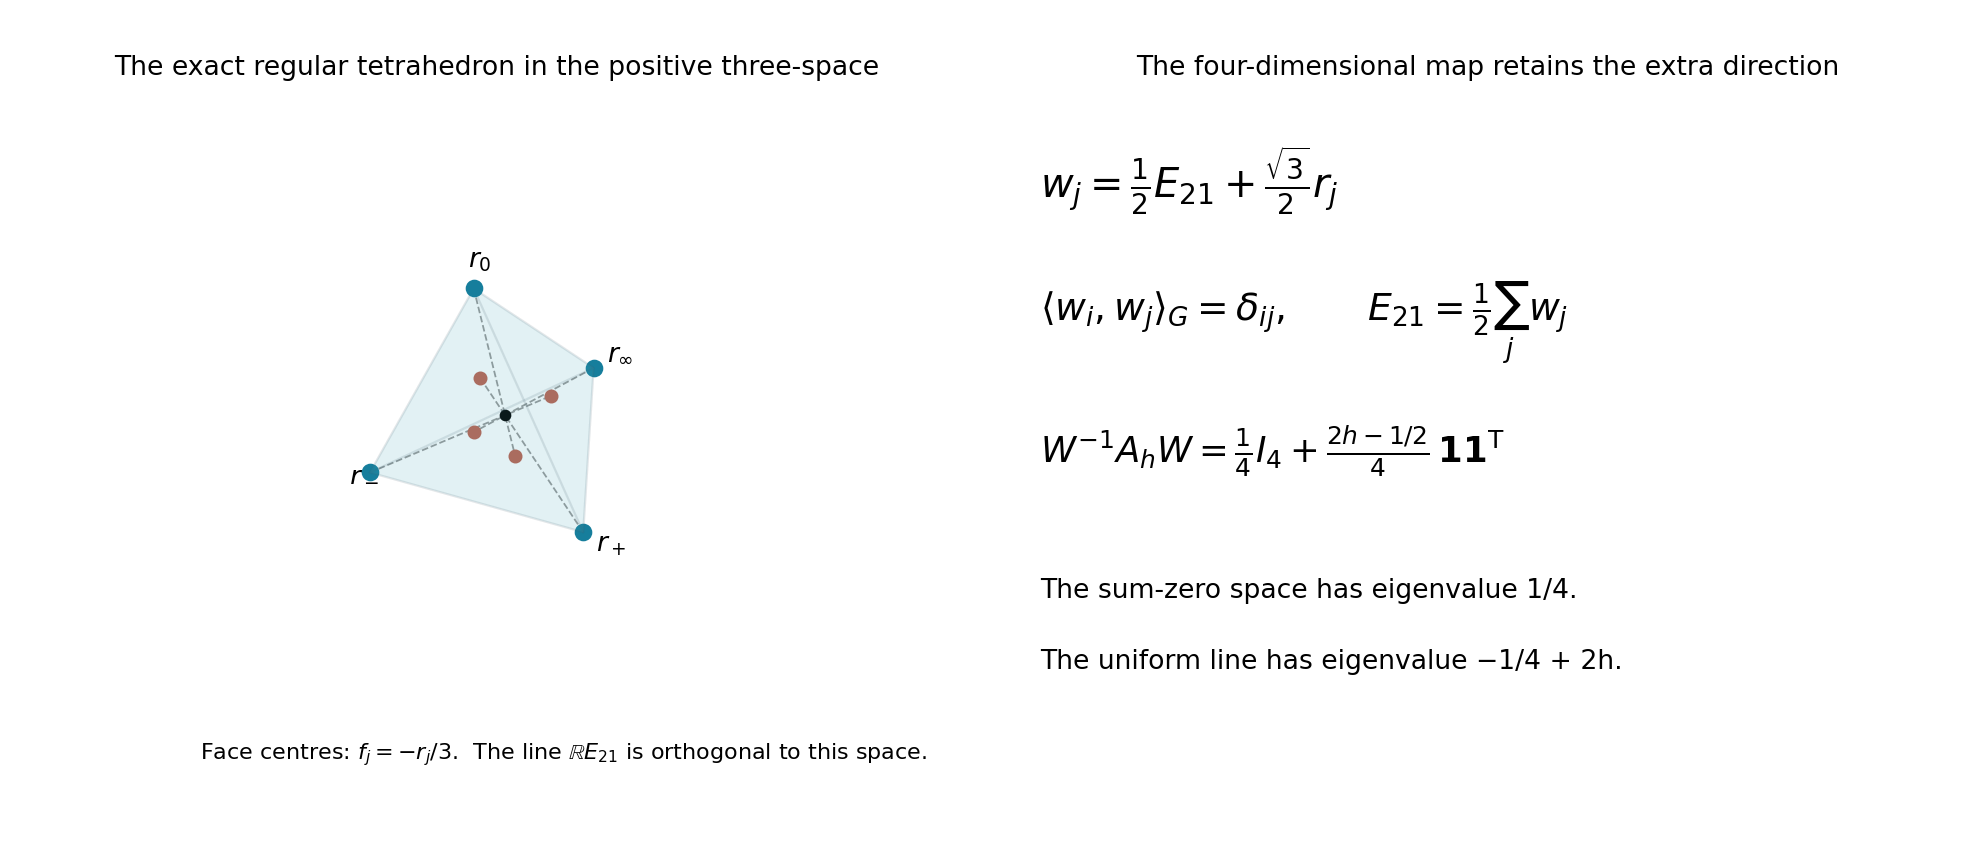
\includegraphics[keepaspectratio,alt={Exact tetrahedral vertices and face centres, with the four-dimensional orthonormal frame. ESQ45--ESQ54 prove the coordinates and the uniform changing direction; the orthogonal E21 direction is retained outside the displayed three-space.}]{figures/27_tetrahedral_heat_frame.png}}
\caption{Exact tetrahedral vertices and face centres, with the
four-dimensional orthonormal frame. ESQ45--ESQ54 prove the coordinates
and the uniform changing direction; the orthogonal E21 direction is
retained outside the displayed three-space.}
\end{figure}

\end{document}
